%%% LaTeX Template: Article/Thesis/etc. with colored headings and special fonts
%%%
%%% Source: http://www.howtotex.com/
%%% Feel free to distribute this template, but please keep to referal to http://www.howtotex.com/ here.
%%% February 2011
%%%
%%% Modified January 2016 by CDM

%%%  Preamble
\documentclass[11pt,letterpaper]{article}
\usepackage[margin=1.0in]{geometry}
\usepackage[T1]{fontenc}
\usepackage[bitstream-charter]{mathdesign}
\usepackage[latin1]{inputenc}					
\usepackage{amsmath}						
\usepackage{xcolor}
\usepackage{cite}
\usepackage{hyphenat}
\usepackage{graphicx}
\usepackage{float}
\usepackage{subfigure}
\usepackage{sectsty}
\usepackage[compact]{titlesec} 
\usepackage[tablegrid]{vhistory}
\usepackage{pbox}
\allsectionsfont{\color{accentcolor}\scshape\selectfont}

%%% Definitions
%%%%%%%%%%%%%%%%%%%%%%%%%%%%%%%%%%%%%%%%%%%%%%%%%%%%
% UPDATE THIS SECTION TO YOUR TEAM AND SEMESTER INFO
\definecolor{accentcolor}{rgb}{0.0,0.0,0.5} 
\newcommand{\teamname}{Runtime Terror}
\newcommand{\productname}{Turing Board}
\newcommand{\coursename}{CSE 4317: Senior Design II}
\newcommand{\semester}{Spring 2022}
\newcommand{\docname}{Detailed Design Specification}
\newcommand{\department}{Department of Computer Science \& Engineering}
\newcommand{\university}{The University of Texas at Arlington}
\newcommand{\authors}{Sahaj Amatya \\ Sarker Nadir Afridi Azmi \\ Kendall Buchanan \\ Keaton Koehler \\ Happy Ndikumnaa \\ Lydia Sarver}

%%% Headers and footers
\usepackage{fancyhdr}
	\pagestyle{fancy}						% Enabling the custom headers/footers
\usepackage{lastpage}	
	% Header (empty)
	\lhead{}
	\chead{}
	\rhead{}
	% Footer
	\lfoot{\footnotesize \teamname \ - \semester}
	\cfoot{}
	\rfoot{\footnotesize page \thepage\ of \pageref{LastPage}}	% "Page 1 of 2"
	\renewcommand{\headrulewidth}{0.0pt}
	\renewcommand{\footrulewidth}{0.4pt}

%%% Change the abstract environment
\usepackage[runin]{abstract}			% runin option for a run-in title
%\setlength\absleftindent{30pt}			% left margin
%\setlength\absrightindent{30pt}		% right margin
\abslabeldelim{\quad}	
\setlength{\abstitleskip}{-10pt}
\renewcommand{\abstractname}{}
\renewcommand{\abstracttextfont}{\color{accentcolor} \small \slshape}	% slanted text

%%% Start of the document
\begin{document}

%%% Cover sheet
%%%%%%%%%%%%%%%%%%%%%%%%%%%%%%%%%%%%%%%%%%%%%%%%%%%%%%%%%%%%%%%%%%%%%%%%%%%%
%   CHANGE THE GRAPHIC HERE. PUT YOUR IMAGE IN THE 'images' 
%   FOLDER AND UPDATE THE NAME FROM 'images/test_image' TO YOUR IMAGE NAME
{\centering \huge \color{accentcolor} \sc \textbf{\department \\ \university} \par}
\vspace{0.5 in}
{\centering \huge \color{accentcolor} \sc \textbf{\docname \\ \coursename \\ \semester} \par}
\vspace{0.3 in}
\begin{figure}[h!]
	\centering
   	
\includegraphics[width=0.60\textwidth]{images/turing_logo} 
\end{figure}
\vspace{0.2 in}
{\centering \huge \color{accentcolor} \sc \textbf{\teamname \\ \productname} \par}
\vspace{0.3 in}
{\centering \large \sc \textbf{\authors} \par}
\newpage


%\vspace{1 in}
%\centerline{January 13th, 2012}
%\newpage

%%% Revision History
%%%%%%%%%%%%%%%%%%%%%%%%%%%%%%%%%%%%%%%%%%%%%%%%%%%%%%%%%%%%%%%%%
%   EACH '\vhEntry' BEGINS A ROW; EACH {} IS A COLUMN. UPDATE
%   THIS TO REFLECT YOUR REVISION HISTORY
\begin{versionhistory}
  	\vhEntry{0.1}{1.01.2016}{GH}{document creation}
  	\vhEntry{0.2}{1.05.2016}{AT|GH}{complete draft}
  	\vhEntry{0.3}{1.12.2016}{AT|GH}{release candidate 1}
  	\vhEntry{1.0}{1.20.2016}{AT|GH|CB}{official release}
  	\vhEntry{1.1}{1.31.2016}{AL}{added design review requests}
\end{versionhistory}
\newpage

%%% Table of contents
\setcounter{tocdepth}{2}
\tableofcontents
\newpage

%%% List of figures and tables (optional)
\listoffigures
\listoftables
\newpage

%%% Document sections
%%%%%%%%%%%%%%%%%%%%%%%%%%%%%%%%%%%%%%%%%%%%%%%%%%%%%%%%%%%%%%%
%   THIS IMPORTS LATEX FILES FROM THE TEX FOLDER. COPY/PASTE TO
%   ADD SECTIONS AS NEEDED AND CREATE FILE FOR IT IN TEX FOLDER
\section{Introduction}
Your introduction should provide a brief overview of the product concept and a reference to the requirement specification and architectural design documents in 1 or 2 paragraphs. The purpose is to provide the reader with the location of relevant background material that lead to the design details presented in this document.

\section{System Overview}
The main controls layer is in charge of processing and sending out the majority of the signals on the Turing Board. It uses the Jetson TX2 to communicate with the microprocessor in the wheels and turning layer to control the wheels and turning mechanism. There are several sensors in the wheels and turning layer that send information via the microprocessor to the Jetson as inputs. The Jetson also receives inputs from the power layer to know how much power is left in the battery. The last input to the Jetson comes from the Human Machine Interface (HMI) layer. This layer consists of items used to allow the Turing Board to understand the world around it and operate more appropriately. Along with the human machine interface layer, the computer vision layer also contributes to the Jetson TX2 receiving feedback from its environment. The computer vision layer uses RGB imagery and stereo and infrared imagery to see obstacles and the user depending on the mode it is currently in. Finally, the remote control for the Turing Board allows the user to control the board as an electric longboard when in the respective mode. The app boasts many features including user authentication and ride data analysis.

%%%%%%%%%%%%%%%%%%%%%%%%%%%%%%%%%%%%%%%%%%%%%%%%%%%%%%%%%%%%%%%%%%%%%%%%%%%%%%%%%%%%%%%%%%%%%
% If you want to change the image, put your image in the images folder and change "data_flow" 
% to the name of your image. You can also change the caption (System architecture) to 
% something else if you want.
\begin{figure}[h!]
	\centering
 	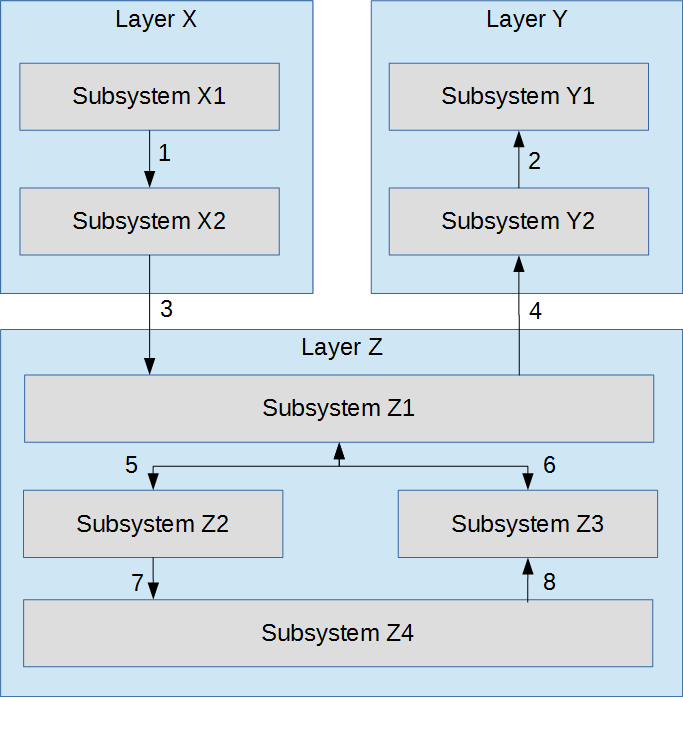
\includegraphics[width=0.90\textwidth]{images/data_flow} % Change me
 \caption{System Architecture}
\end{figure}

\newpage
%\section{Subsystem Definitions \& Data Flow}
%This section breaks down your layer abstraction to another level of detail. Here you grapically represent the logical subsytems that compose each layer and show the interactions/interfaces between those subsystems. A subsystem can be thought of as a programming unit that implements one of the major functions of the layer. It, therefore, has data elements that serve as source/sinks for other subsystems. The logical data elements that flow between subsystems need to be explicitly defined at this point, beginning with a data flow-like diagram based on the block diagram.

%%%%%%%%%%%%%%%%%%%%%%%%%%%%%%%%%%%%%%%%%%%%%%%%%%%%%%%%%%
%  BE SURE TO UPDATE THE IMAGE CAPTION
\begin{figure}[h!]
	\centering
 	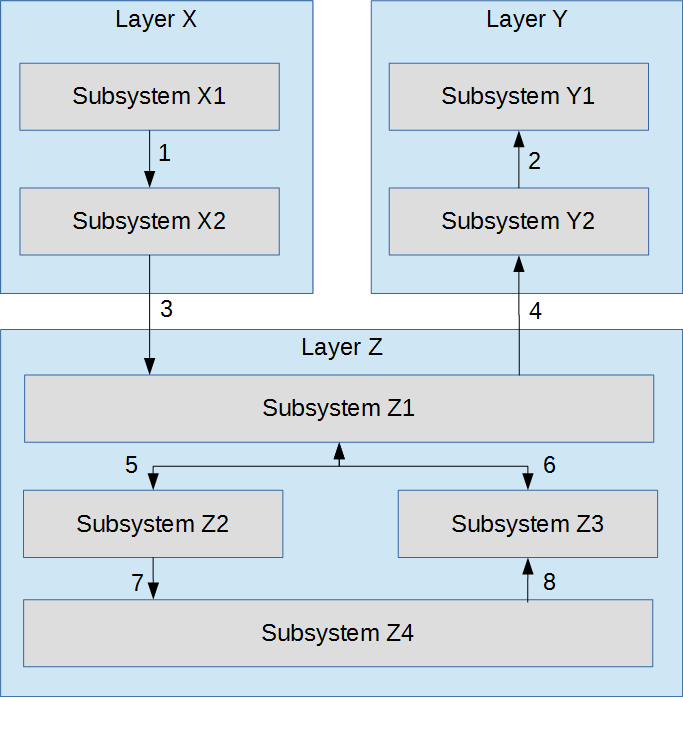
\includegraphics[width=\textwidth]{images/data_flow} % Image
 \caption{A simple data flow diagram} % Caption
\end{figure}

\newpage
\section{X Layer Subsystems}
In this section, the layer is described in terms of the hardware and software design. Specific implementation details, such as hardware components, programming languages, software dependencies, operating systems, etc. should be discussed. Any unnecessary items can be omitted (for example, a pure software module without any specific hardware should not include a hardware subsection). The organization, titles, and content of the sections below can be modified as necessary for the project.

\subsection{Layer Hardware}
A description of any involved hardware components for the layer. For example, if each subsystem is a software process running on an embedded computer, discuss the specifics of that device here. Do not list a hardware component that only exists at the subsystem level (include it in the following sections).

\subsection{Layer Operating System}
A description of any operating systems required by the layer.

\subsection{Layer Software Dependencies}
A description of any software dependencies (libraries, frameworks, etc) required by the layer.

\subsection{Subsystem 1}
Describe at a high level the purpose and basic design of this subsystem. Is it a piece of hardware, a class, a web service, or something else? Note that each of the subsystem items below are meant to be specific to that subsystem and not a repeat of anything discussed above for the overall layer.

%%%%%%%%%%%%%%%%%%%%%%%%%%%%%%%%%%%%%%%%%%%%%%%%%%%%%%%%%%
%  BE SURE TO UPDATE THE IMAGE CAPTION
\begin{figure}[h!]
	\centering
 	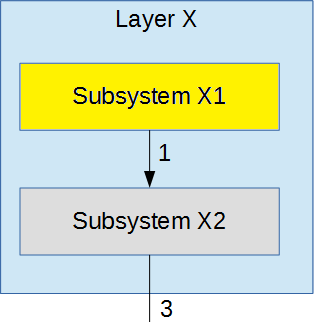
\includegraphics[width=0.60\textwidth]{images/subsystem} % Image
 \caption{Example subsystem description diagram} % Caption
\end{figure}

\subsubsection{Subsystem Hardware}
A description of any involved hardware components for the subsystem.

\subsubsection{Subsystem Operating System}
A description of any operating systems required by the subsystem.

\subsubsection{Subsystem Software Dependencies}
A description of any software dependencies (libraries, frameworks, design software for mechanical parts or circuits, etc) required by the subsystem.

\subsubsection{Subsystem Programming Languages}
A description of any programming languages used by the subsystem.

\subsubsection{Subsystem Data Structures}
A description of any classes or other data structures that are worth discussing for the subsystem. For example, data being transmitted from a microcontroller to a PC via USB should be first be assembled into packets. What is the structure of the packets?

\subsubsection{Subsystem Data Processing}
A description of any algorithms or processing strategies that are worth discussing for the subsystem. If you are implementing a well-known algorithm, list it. If it is something unique to this project, discuss it in greater detail.



\newpage
\section{Y Layer Subsystems}
In this section, the layer is described in terms of the hardware and software design. Specific implementation details, such as hardware components, programming languages, software dependencies, operating systems, etc. should be discussed. Any unnecessary items can be omitted (for example, a pure software module without any specific hardware should not include a hardware subsection). The organization, titles, and content of the sections below can be modified as necessary for the project.

\subsection{Layer Hardware}
A description of any involved hardware components for the layer. For example, if each subsystem is a software process running on an embedded computer, discuss the specifics of that device here. Do not list a hardware component that only exists at the subsystem level (include it in the following sections).

\subsection{Layer Operating System}
A description of any operating systems required by the layer.

\subsection{Layer Software Dependencies}
A description of any software dependencies (libraries, frameworks, etc) required by the layer.

\subsection{Subsystem 1}
Describe at a high level the purpose and basic design of this subsystem. Is it a piece of hardware, a class, a web service, or something else? Note that each of the subsystem items below are meant to be specific to that subsystem and not a repeat of anything discussed above for the overall layer.

%%%%%%%%%%%%%%%%%%%%%%%%%%%%%%%%%%%%%%%%%%%%%%%%%%%%%%%%%%
%  BE SURE TO UPDATE THE IMAGE CAPTION
\begin{figure}[h!]
	\centering
 	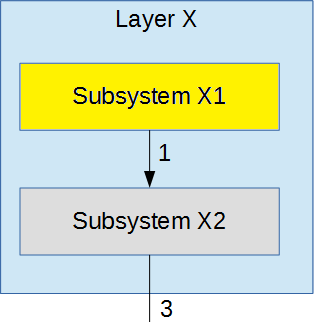
\includegraphics[width=0.60\textwidth]{images/subsystem} % Image
 \caption{Example subsystem description diagram} % Caption
\end{figure}

\subsubsection{Subsystem Hardware}
A description of any involved hardware components for the subsystem.

\subsubsection{Subsystem Operating System}
A description of any operating systems required by the subsystem.

\subsubsection{Subsystem Software Dependencies}
A description of any software dependencies (libraries, frameworks, design software for mechanical parts or circuits, etc) required by the subsystem.

\subsubsection{Subsystem Programming Languages}
A description of any programming languages used by the subsystem.

\subsubsection{Subsystem Data Structures}
A description of any classes or other data structures that are worth discussing for the subsystem. For example, data being transmitted from a microcontroller to a PC via USB should be first be assembled into packets. What is the structure of the packets?

\subsubsection{Subsystem Data Processing}
A description of any algorithms or processing strategies that are worth discussing for the subsystem. If you are implementing a well-known algorithm, list it. If it is something unique to this project, discuss it in greater detail.



\newpage
\section{Z Layer Subsystems}
In this section, the layer is described in terms of the hardware and software design. Specific implementation details, such as hardware components, programming languages, software dependencies, operating systems, etc. should be discussed. Any unnecessary items can be omitted (for example, a pure software module without any specific hardware should not include a hardware subsection). The organization, titles, and content of the sections below can be modified as necessary for the project.

\subsection{Layer Hardware}
A description of any involved hardware components for the layer. For example, if each subsystem is a software process running on an embedded computer, discuss the specifics of that device here. Do not list a hardware component that only exists at the subsystem level (include it in the following sections).

\subsection{Layer Operating System}
A description of any operating systems required by the layer.

\subsection{Layer Software Dependencies}
A description of any software dependencies (libraries, frameworks, etc) required by the layer.

\subsection{Subsystem 1}
Describe at a high level the purpose and basic design of this subsystem. Is it a piece of hardware, a class, a web service, or something else? Note that each of the subsystem items below are meant to be specific to that subsystem and not a repeat of anything discussed above for the overall layer.

%%%%%%%%%%%%%%%%%%%%%%%%%%%%%%%%%%%%%%%%%%%%%%%%%%%%%%%%%%
%  BE SURE TO UPDATE THE IMAGE CAPTION
\begin{figure}[h!]
	\centering
 	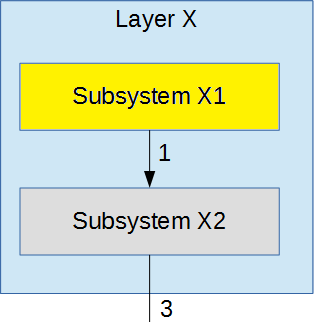
\includegraphics[width=0.60\textwidth]{images/subsystem} % Image
 \caption{Example subsystem description diagram} % Caption
\end{figure}

\subsubsection{Subsystem Hardware}
A description of any involved hardware components for the subsystem.

\subsubsection{Subsystem Operating System}
A description of any operating systems required by the subsystem.

\subsubsection{Subsystem Software Dependencies}
A description of any software dependencies (libraries, frameworks, design software for mechanical parts or circuits, etc) required by the subsystem.

\subsubsection{Subsystem Programming Languages}
A description of any programming languages used by the subsystem.

\subsubsection{Subsystem Data Structures}
A description of any classes or other data structures that are worth discussing for the subsystem. For example, data being transmitted from a microcontroller to a PC via USB should be first be assembled into packets. What is the structure of the packets?

\subsubsection{Subsystem Data Processing}
A description of any algorithms or processing strategies that are worth discussing for the subsystem. If you are implementing a well-known algorithm, list it. If it is something unique to this project, discuss it in greater detail.



\newpage
\section{Appendix A}
Include any additional documents (CAD design, circuit schematics, etc) as an appendix as necessary.
\newpage

%%% References
\bibliographystyle{plain}
\bibliographystyle{reference/IEEEtran_custom}
\bibliography{reference/refs}{}

\end{document}